%!TEX root=../GaugeCNNTheory.tex


\subsection
[هندسه‌ی آفین فضاهای اقلیدسی \texorpdfstring{$\Euc_d$}{}]%
{هندسه‌ی آفین فضاهای اقلیدسی $\Euc_d$}
\label{sec:euclidean_geometry}


قبل از بحث در مورد کانولوشن‌های مستقل از مختصات در فضاهای اقلیدسی، باید هندسه‌ی اقلیدسی زیربنایی را درک کنیم.
فضاهای اقلیدسی $\Euc_d$ بنا به تعریف، فضاهای \emph{آفین} هستند، یعنی با یک فضای برداری متناظر با بعد $d$ همراه هستند که \emph{انتقال‌ها} را روی~$\Euc_d$ تعریف می‌کند.
فضاهای اقلیدسی علاوه بر اینکه فضای آفین هستند، به یک \emph{متریک اقلیدسی} (تابع فاصله) نیز مجهزند.
این تابع فاصله متناظر با یک متریک ریمانی $\eta$ است، یعنی یک $\O{d}$-ساختار $\OM$ روی منیفلد (ریمانی) $M=\Euc_d$.
این متریک دارای این ویژگی است که انحنای آن در همه جا صفر است، یعنی $\Euc_d$ سرتاسر تخت است.


یک مثال استاندارد برای فضاهای اقلیدسی، \emph{فضاهای برداری} $\R^d$ هستند، با این حال، فضاهای اقلیدسی عمومی ساختار کمتری را در نظر می‌گیرند.
به طور خاص، آنها با یک ساختار فضای برداری همراه نیستند و بنابراین مبدأ مرجحی ندارند.
علاوه بر این، آنها به طور کلی مجهز به مختصات دکارتی نیستند.
بنابراین ما با فضاهای اقلیدسی «عریان» $\Euc_d$ شروع می‌کنیم و بحث می‌کنیم که چگونه ساختار هندسی مربوطه به آنها اضافه می‌شود.
در اصل می‌توان هر $G$-ساختاری را در نظر گرفت، با این حال، ما به طور خاص به آن $G$-ساختارهایی علاقه‌مندیم که \lr{CNN}های راهبری‌پذیر کلاسیک را از بخش قبل بازیابی می‌کنند، که تمام مدل‌های ردیف‌های (۱-۲۶) جدول~\ref{tab:network_instantiations} را توضیح می‌دهają.
چنین $G$-ساختارهای ناوردای $\Aff(G)$ از اطلس‌های $\Aff(G)$ القا می‌شوند، که شامل چارت‌هایی از $\Euc_d$ هستند که توابع گذار آنها مقادیری در $\Aff(G)$ می‌گیرند (معادله~\eqref{eq:AffG_def})؛ به شکل~\ref{fig:affine_charts} مراجعه کنید.
تمام گزاره‌هایی که در مختصات $\R^d$ بیان می‌شوند، می‌توانند از طریق چارت‌ها به یک چارچوب مستقل از مختصات ترجمه شوند، که ما در اینجا آن را توسعه می‌دهیم.
اطلاعات بیشتر در مورد رابطه بین چارت‌های مختصاتی و پیمانه‌ها را می‌توان در پیوست~\ref{apx:coordinate_bases} یافت.

\begin{figure}
	\centering
	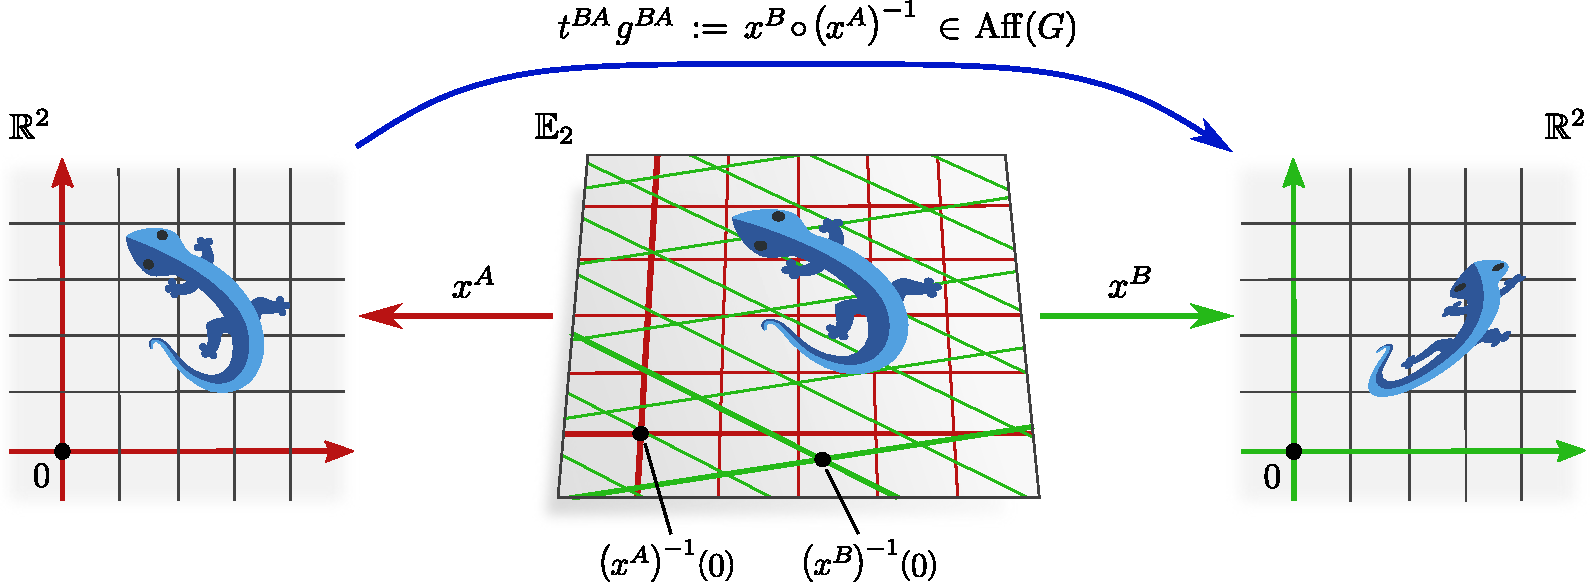
\includegraphics[width=1.\textwidth]{figures/affine_charts.pdf}
	\vspace*{2ex}
	\caption{\small
		نمایش چارت‌های آفین $x^X: \Euc_d \to \R^d$ که مختصات سراسری را به فضاهای اقلیدسی اختصاص می‌دهند.
		هم $\Euc_d$ و هم $\R^d$ فضاهای آفین هستند، به طوری که می‌توان خواست که چارت‌ها نگاشت‌های آفین باشند، که هم‌خطی و نسبت فاصله‌ها را حفظ می‌کنند.
		ما یک اطلس $\Aff(G)$ با نماد $\mathscr{A}^{\Aff(G)}_{\Euc_d}$ را به عنوان اطلسی متشکل از چارت‌هایی تعریف می‌کنیم که توسط توابع گذار $t^{BA} g^{BA} := x^B \circ (x^A)^{-1}$ که اعضایی در $\Aff(G)$ هستند، به یکدیگر مرتبط می‌شوند.
		چارت‌ها در یک اطلس $\Aff(G)$ حداکثر در انتخاب مبدأ $(x^X)^{-1}(0)$ و یک تبدیل $G$ با هم تفاوت دارند.
		انتخاب یک اطلس $\Aff(G)$، متشکل از چارت‌های $x^X$، یک $G$-اطلس $\mathscr{A}^G$ از پیمانه‌های $\hat{d}x^X$ را القا می‌کند.
		$G$-ساختار متناظر $\GM$ که در شکل~\ref{fig:G_structures_R2_main} برای گروه‌های مختلف $G$ مثال زده شده است، تحت عمل $\Aff(G)$ ناوردا است.
		قضیه~\ref{thm:affine_equivariance_Euclidean_GM_conv} ثابت می‌کند که کانولوشن‌های $\GM$ روی چنین $G$-ساختارهایی، $\Aff(G)$-هموردا هستند.
		{\\
			\color{gray}
			\scriptsize
			(مارمولک‌ها با مجوز توییتر تحت لایسنس بین‌المللی 
			Creative Commons Attribution 4.0 
			\href{https://github.com/twitter/twemoji/blob/gh-pages/LICENSE-GRAPHICS}{\underline{license}}
			اقتباس شده‌اند.)
		}
	}
	\label{fig:affine_charts}
\end{figure}


\subsubsection{چارت‌های آفین و اطلس‌های \lr{Aff(G)}}
یک فضای اقلیدسی $\Euc_d$ با بعد $d$ با $\R^d$ همسان‌ریخت است و بنابراین چارت‌های سراسری را می‌پذیرد%
\footnote{
	این واقعیت که $\Euc_d$ و $\R^d$ به صورت سراسری همسان‌ریخت (یا حتی ایزومتریک) هستند، توضیح می‌دهد که چرا اکثر کارهای مرتبط، فضاهای برداری $\R^d$ را به عنوان مدل‌هایی از فضاهای اقلیدسی در نظر می‌گیرند.
	رویکرد ما در این بخش کمی دقیق‌تر است زیرا حداقل ساختار لازم برای تعریف کانولوشن‌های مستقل از مختصات $\GM$ را در فضاهای اقلیدسی $M=\Euc_d$ معرفی می‌کند.
}
\begin{align}
	x^A: \Euc_d \to \R^d \,.
\end{align}
در ادامه ما همیشه این چارت‌ها را به عنوان نگاشت‌های آفین، یعنی ایزومورفیسم‌های فضاهای آفین، که هم‌خطی (یعنی خطوط راست را به خطوط راست می‌نگارند) و نسبت فاصله‌ها را حفظ می‌کنند، در نظر خواهیم گرفت.
از آنجا که ترکیب نگاشت‌های آفین، خود نگاشت آفین است، نتیجه می‌شود که توابع گذار چارت
\begin{align}
	x^B \mkern-1mu\circ\mkern-1mu \big(x^A \big)^{-1}:\ \R^d \to \R^d
\end{align}
تبدیلات آفین از $\R^d$ هستند، یعنی اعضایی در $\Aff(\GL{d})$.
بنابراین توابع گذار به طور یکتا به یک انتقال $t^{BA} \in \Trans_d$ و یک عضو $g^{BA} \in \GL{d}$ تجزیه می‌شوند:
\begin{align}
	t^{BA} g^{BA}\ :=\ x^B \mkern-1mu\circ\mkern-1mu \big(x^A \big)^{-1}
\end{align}
نماد $g^{BA}$ در اینجا تصادفی نیست زیرا این اعضای گروه با تبدیلات پیمانه‌ای که توسط گذار چارت‌ها القا می‌شوند، مطابقت دارند، که در قضیه~\ref{thm:AffG_atlas_induced_G_atlas} در ادامه ثابت شده است.

با توجه به انتخاب یک گروه آفین $\Aff(G)$، ما اطلس‌های $\Aff(G)$ از $\Euc_d$ را به عنوان آن دسته از اطلس‌های چارت‌های سراسری از $\Euc_d$ به $\R^d$ تعریف می‌کنیم که توابع گذار چارت آنها مقادیری در $\Aff(G)$ می‌گیرند:
\begin{dfn}[اطلس $\Aff(G)$ از فضای اقلیدسی]
	\label{dfn:AffG_atlas}
	فرض کنید $\mathfrak{X}$ یک مجموعه اندیس برای نام‌گذاری چارت‌ها باشد و برای هر ${X \mkern-2mu\in \mathfrak{X}}$، $x^X: \Euc_d \to \R^d$ یک چارت آفین سراسری از $\Euc_d$ باشد.
	اطلس
	\begin{align}
		\mathscr{A}^{\Aff(G)}_{\Euc_d}\ =\ \pig\{ \big( \Euc_d, x^X \big) \;\pig|\ X\in \mathfrak{X} \,\pig\}
	\end{align}
	یک اطلس $\Aff(G)$ نامیده می‌شود اگر تمام توابع گذار چارت آن مقادیری در $\Aff(G)$ بگیرند، یعنی اگر
	\begin{align}
		x^B \mkern-3mu\circ\mkern-2mu \big(x^A\big)^{-1} \!\in \Aff(G) \quad \forall\ A,B \in \mathfrak{X} \,.
	\end{align}
\end{dfn}
شکل~\ref{fig:affine_charts} چارت‌های آفین و نگاشت‌های گذار چارت با مقادیر $\Aff(G)$ بین آنها را به تصویر می‌کشد.


\subsubsection{\textit{G}-اطلس‌ها و \textit{G}-ساختارهای القا شده}
هر چارت مختصاتی سراسری $x^A: \Euc_d \to \R^d$ یک پیمانه سراسری را القا می‌کند که به صورت نقطه‌ای توسط گرادیان‌های چارت داده می‌شود
\begin{align}
	\psiTMp^A := \hat{d}x_p^A :\ \TpM \to \R^d \,,
\end{align}
به معادله~\eqref{eq:chart_differential_via_gradients} در پیوست~\ref{apx:chart_induced_bases_main} و جدول~\ref{tab:coord_charts_gauge_trafos} مراجعه کنید.
بنابراین یک اطلس از چارت‌ها متناظر با یک اطلس از پیمانه‌ها است.
به طور خاص، با توجه به اینکه چارت‌ها یک اطلس $\Aff(G)$ را تشکیل می‌دهند، تضمین می‌شود که تبدیلات پیمانه دارای مقادیر $G$ هستند، یعنی پیمانه‌های القا شده یک $G$-اطلس را تشکیل می‌دهند:
\begin{thm}[اطلس‌های $\Aff(G)$ از چارت‌ها، $G$-اطلس‌هایی از پیمانه‌ها را القا می‌کنند]
	\label{thm:AffG_atlas_induced_G_atlas}
	فرض کنید ${\mathscr{A}^{\Aff(G)}_{\Euc_d} \!= \big\{ ( \Euc_d, x^X ) \big| X \mkern-2mu\in\mkern-2mu \mathfrak{X} \big\}}$ یک اطلس $\Aff(G)$ از \emph{چارت‌ها} باشد.
	اطلس القا شده از \emph{پیمانه‌ها}
	\begin{align}
		\mathscr{A}^G = \pig\{ \big(\Euc_d, \hat{d}x^X \big) \,\pig|\, X \in \mathfrak{X} \pig\}
	\end{align}
	تضمین می‌شود که یک $G$-اطلس باشد.
	به طور خاص، اگر نگاشت‌های گذار چارت با ${x^B \circ (x^A)^{-1}} = t^{BA} g^{BA}$ داده شوند، نگاشت‌های گذار بین پیمانه‌ها در هر نقطه $p\in \Euc_d$ با ${g_p^{BA} = g^{BA} \in G}$ داده می‌شوند.
\end{thm}
\begin{proof}
	توابع گذار بین پیمانه‌های القا شده توسط چارت، طبق معادله~\eqref{eq:chart_differential_trafo_law}، با ژاکوبین نگاشت‌های گذار چارت منطبق هستند، یعنی،
	\begin{align}
		g_p^{BA} \,=\, \hat{d}x^B_p \circ \big(\hat{d}x^A_p \big)^{-1} \,=\, \frac{\partial x^B}{\partial x^A} \Big|_{x^A(p)} \,.
	\end{align}
	عبارت آخر، سوءاستفاده معمول از نمادگذاری برای ژاکوبین‌های نگاشت‌های گذار چارت است، که در معادله~\eqref{eq:abuse_of_notation_jacobian} به صورت مؤلفه‌ای به شکل زیر تعریف شد:
	\begin{align}
		\frac{\partial x^B_\mu}{\partial x^A_\nu} \bigg|_{x^A(p)}
		\,:=\,
		\partial_\nu \pig(x^B_\mu \circ \big(x^A\big)^{-1} \pig) \Big|_{x^A(p)} \,.
	\end{align}
	با استفاده از اینکه نگاشت‌های گذار چارت با $x^B \circ \big(x^A\big)^{-1} = t^{BA} g^{BA}$ داده می‌شوند، این نتیجه می‌دهد که
	\begin{align}
		\big( g_p^{BA} \big)_{\mu\nu}
		\ =\ \partial_\nu \pig(x^B_\mu \circ \big(x^A\big)^{-1} \pig) (\mathscr{x}) \big|_{x^A(p)}
		\ =\ \partial_\nu \big( g^{BA} \mathscr{x} + t^{BA} \big)_\mu \big|_{x^A(p)}
		\ =\ g^{BA}_{\mu\nu} \,,
	\end{align}
	یعنی تبدیلات پیمانه القا شده $g_p^{BA}$ مقادیری در $G$ دارند و با $g^{BA}$ مطابقت دارند (که این نمادگذاری را توجیه می‌کند).
	از آنجا که این استدلال برای هر $p\in \Euc_d$ و هر چارت $A,B \in \mathfrak{X}$ برقرار است، نتیجه می‌شود که اطلس القا شده از پیمانه‌ها یک $G$-اطلس است.
\end{proof}


\begin{figure}
	\centering
	\begin{subfigure}[b]{0.46\textwidth}
		\centering
		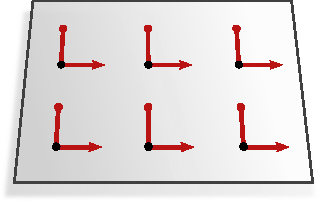
\includegraphics[width=.7\textwidth]{figures/G_structure_R2_1.pdf}
		\captionsetup{format=hang}
		\caption{\small
			$\{e\}$-ساختار $\eM$ القا شده توسط اطلس $\Aff(\{e\})$ روی ${M=\Euc_2}$، که تحت \emph{انتقال‌ها} در $\Aff(\{e\}) = \IsomeM = \Trans_2$ حفظ می‌شود.
		}
		\label{fig:G_structure_R2_1}
	\end{subfigure}
	\hfill
	\begin{subfigure}[b]{0.46\textwidth}
		\centering
		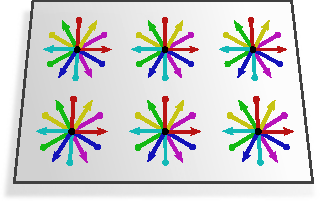
\includegraphics[width=.7\textwidth]{figures/G_structure_R2_2.pdf}
		\captionsetup{format=hang}
		\caption{\small
			$\SO2$-ساختار $\SOM$ القا شده توسط اطلس $\Aff(\SO2)$ روی $M=\Euc_2$، که تحت \emph{انتقال‌ها} و \emph{دوران‌ها} در $\Aff(\SO2) = \IsomSOM = \SE2$ حفظ می‌شود.
		}
		\label{fig:G_structure_R2_2}
	\end{subfigure}
	\\[3ex]
	\begin{subfigure}[b]{0.46\textwidth}
		\centering
		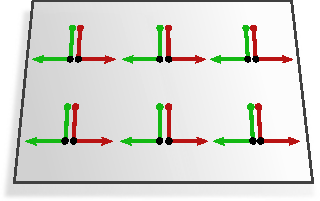
\includegraphics[width=.7\textwidth]{figures/G_structure_R2_3.pdf}
		\captionsetup{format=hang}
		\caption{\small
			$\Flip$-ساختار $\RM$ القا شده توسط اطلس $\Aff(\Flip)$ روی $M=\Euc_2$، که تحت \emph{انتقال‌ها} و \emph{بازتاب‌ها} در $\Aff(\Flip) = \IsomRM = \Trans_2 \rtimes \Flip$ حفظ می‌شود.
			\\
		}
		\label{fig:G_structure_R2_3}
	\end{subfigure}
	\hfill
	\begin{subfigure}[b]{0.46\textwidth}
		\centering
		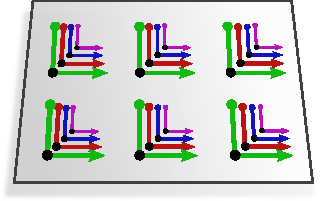
\includegraphics[width=.7\textwidth]{figures/G_structure_R2_4.pdf}
		\captionsetup{format=hang}
		\caption{\small
			$\Scale$-ساختار $\SM$ القا شده توسط اطلس $\Aff(\Scale)$ روی $M=\Euc_2$، که تحت \emph{انتقال‌ها} و \emph{مقیاس‌بندی‌ها} در $\Aff(\Scale) = \Trans_2 \rtimes \Scale$ حفظ می‌شود.
			توجه داشته باشید که $\IsomSM = \Trans_2$ زیرا مقیاس‌بندی‌ها ایزومتریک نیستند.
		}
		\label{fig:G_structure_R2_4}
	\end{subfigure}
	\vspace*{0ex}
	\caption{\small
		نمایش $G$-ساختارهای مختلف $\GM$ در فضاهای اقلیدسی $M=\Euc_2$ که توسط یک اطلس $\Aff(G)$ از چارت‌ها القا می‌شوند (تعریف~\ref{dfn:AffG_atlas}).
		شکل~\ref{fig:G_structure_R2_1} $\{e\}$-ساختار ناوردای انتقالی $\eM$ را نشان می‌دهد که متناظر با کانولوشن‌های اقلیدسی متعارف است.
		سه $G$-ساختار دیگر متناظر با \lr{CNN}های $G$-راهبری‌پذیر غیربدیهی هستند.
		آنها به صورت محلی روی تمام ژست‌هایی که توسط مجموعه خاصی از چارچوب‌های مرجع در $\GpM$ به هم مرتبط هستند، تعمیم می‌یابند.
		از آنجا که $G$-ساختارها $\Aff(G)$-ناوردا هستند (که از قضیه~\ref{thm:Aff_GM_in_charts} نتیجه می‌شود)، کانولوشن‌های $G$-راهبری‌پذیر به صورت سراسری نسبت به $\Aff(G)$ هموردا هستند (قضیه~\ref{thm:affine_equivariance_Euclidean_GM_conv}).
		به جای تعریف $G$-ساختارها از طریق یک اطلس $\Aff(G)$ از چارت‌ها، می‌توان آنها را از طریق یک ارتقای-$G$ به صورت $\GM := \eM \lhd G$ از $\{e\}$-ساختار کانونیِ $\R^d$ تعریف کرد (معادله~\eqref{eq:G_lifted_G_structure_Rd})، که چارچوب‌های موجود در $\{e\}$-ساختار را با تمام چارچوب‌های مرتبط با $G$ مجهز می‌کند.
	}
	\label{fig:G_structures_R2_main}
\end{figure}


همانطور که در بخش~\ref{sec:bundle_trivializations} بحث شد، هر $G$-اطلس از پیمانه‌ها یک $G$-ساختار $\GM$ را القا می‌کند.
طبق معادله~\eqref{eq:G_atlas_induced_G_structure_GM_def_ptwise}، $\GM$ به صورت نقطه‌ای توسط
\begin{align}
	\GpM\ :=\ \big( \psiFMp^A \big)^{-1} (G) \,,
\end{align}
تعیین می‌شود، که در آن انتخاب خاص پیمانه $A \in \mathfrak{X}$ دلخواه است.
چارچوب‌های موجود در $\GpM$ پایه‌های مختصاتی
$\big[ \frac{\partial}{\partial x^A_\mu} \big|_p \big]_{\mu=1}^d = \big[\big(\hat{d}x_p^A \big)^{-1} (\epsilon_\mu) \big]_{\mu=1}^d$
و تمام تبدیلات $G$ آنها هستند.
از آنجا که اطلس ماکسیمال $\Aff(G)$ بنا به تعریف $\Aff(G)$-ناوردا است، همین امر برای $G$-ساختار القا شده نیز صادق است (با عملی که از طریق هر چارت تعریف می‌شود، همانطور که در ادامه روشن و اثبات شده است).
شکل~\ref{fig:G_structures_R2_main} چنین $G$-ساختارهایی را برای گروه‌های آفین مختلف نشان می‌دهد.
در بخش بعدی ما ثابت می‌کنیم که کانولوشن‌های $\GM$ متناظر، تحت عمل~$\Aff(G)$ هموردا هستند.


همانطور که مشخص می‌شود، $\GM \xrightarrow{\piGM} \Euc_d$ به عنوان یک کلاف اصلی با $\Aff(G) \xrightarrow{\mathscr{q}} \Aff(G)/G \cong \R^d$ (به‌صورت غیرکانونی) ایزومورف است، که در آن
\begin{align}
	\mathscr{q}:\ \Aff(G) \to \R^d,\ \ tg \mapsto t
\end{align}
نگاشت خارج‌قسمتی کانونی گروه آفین است (پس از یکی گرفتن هم‌دسته‌های $tG$ با انتقال‌های $t$).%
\footnote{
	ما به طور ضمنی از یک ایزومورفیسم کانونی $\Aff(G)/G \xrightarrow{\sim} \R^d,\ \ tG \mapsto t$ استفاده می‌کنیم، که در آن $t$ در سمت چپ یک عضو گروه انتقال در $\Trans_d = (\R^d,+)$ و در سمت راست یک بردار در $\R^d$ را نشان می‌دهد.
}
جای تعجب نیست که این ایزومورفیسم کلاف اصلی به انتخاب چارت بستگی دارد.

\begin{thm}[ایزومورفیسم کلاف اصلی بین \lr{Aff(G)} و \textit{GM}]
	\label{thm:principal_bundle_isomorphism}
	فرض کنید $\GM$ یک $G$-ساختار القا شده توسط اطلس $\Aff(G)$ روی $\Euc_d$ باشد.
	آنگاه $\GM$ به عنوان یک کلاف اصلی با $\Aff(G) \xrightarrow{\mathscr{q}} \R^d$ ایزومورف است، یعنی ایزومورفیسم‌هایی وجود دارند
	\begin{align}\label{eq:principal_bundle_iso_AffG_GM}
		\alpha^A: \Aff(G) \to \GM,\ \ tg \mapsto \big( \psiGMxAinvt \big)^{-1}(g)
	\end{align}
	و
	\begin{align}
		\big( x^A \big)^{-1}: \R^d \to \Euc_d
	\end{align}
	به طوری که نمودار زیر جابجایی است:
	\begin{equation}\label{cd:GM_def_embedding}
		\begin{tikzcd}[row sep=2.5em, column sep=7.em]
			\Aff(G) \times G
			\arrow[r, "{\alpha^A \times \id_G}"]
			\arrow[d, "{\cdot}"']
			& \GM \times G
			\arrow[d, "{\,\lhd}"]
			\\
			\Aff(G)
			\arrow[r, pos=.5, "{\alpha^A}"]
			\arrow[d, "{\mathscr{q}}"']
			& \GM
			\arrow[d, "{\,\piGM}"]
			\\
			\R^d
			\arrow[r, pos=.55, "{(x^A)^{-1}}"']
			& \Euc_d
		\end{tikzcd}
	\end{equation}
	وارون $\alpha^A$ در اینجا با
	\begin{equation}
		\big(\alpha^A \big)^{-1}: \GM \to \Aff(G),\ \ [e_i]_{i=1}^d \mapsto tg
		\quad \textup{where} \quad
		\begin{cases}
			t = x^A \circ \piGM \big( [e_i]_{i=1}^d \big) \\[1ex]
			g = \psi_{\protect\scalebox{.6}{$G\!M,$}\protect\scalebox{.7}{$\piGM([e_i]_{i=1}^d)$}}^A \big( [e_i]_{i=1}^d \big)
		\end{cases}
	\end{equation}
	داده می‌شود. توجه داشته باشید که این ایزومورفیسم‌ها در تناظر یک به یک با چارت‌های سازگار با $\Aff(G)$ از اطلس مورد نظر هستند.
\end{thm}

\begin{proof}
	برای اثبات این گزاره، باید نشان دهیم که $\alpha^A$ و $(\alpha^A)^{-1}$ واقعاً وارون یکدیگر هستند، که $\alpha^A$ یک نگاشت کلاف روی $(x^A)^{-1}$ است و $\alpha^A$ هموردای-راست نسبت به $G$ است.
	اینکه $(\alpha^A)^{-1}$ هم یک وارون چپ و هم یک وارون راست خوش‌تعریف برای $\alpha^A$ است، به راحتی توسط خواننده بررسی می‌شود.
	اینکه $\alpha^A$ یک نگاشت کلاف روی $(x^A)^{-1}$ است به این معناست که مربع پایینی نمودار جابجایی است.
	این امر با مشاهده اینکه
	$(x^A)^{-1} \circ \mathscr{q} (tg) = (x^A)^{-1} (t)$ و
	$\piGM \circ \alpha^A (tg) = \piGM \circ \big(\psiGMxAinvt \big)^{-1}(g) = (x^A)^{-1} (t)$
	برای هر $tg \in \Aff(G)$ برابر هستند، دیده می‌شود.
	جابجایی مربع بالایی در نمودار، یعنی هموردایی-راست $\alpha^A$ نسبت به $G$، از این واقعیت ناشی می‌شود که
	$\alpha^A (tg \cdot \tilde{g}) = \big(\psiGMxAinvt \big)^{-1}(g \tilde{g}) = \big(\psiGMxAinvt \big)^{-1}(g) \lhd \tilde{g} = \alpha^A(tg) \lhd \tilde{g}$
	برای هر $tg\in \Aff(G)$ و هر $\tilde{g} \in G$ برقرار است.
	در مرحله دوم از این واقعیت استفاده شد که $\psiGMxAinvt$ هموردای-راست نسبت به $G$ است (معادله~\eqref{eq:right_equivariance_GM})، که هموردایی وارون آن را نتیجه می‌دهد.
	در مجموع، این ویژگی‌ها نشان می‌دهند که $\alpha^A$ یک ایزومورفیسم کلاف اصلی است.
\end{proof}




\subsubsection{تبدیلات آفین مستقل از مختصات}
از آنجا که ما می‌خواهیم هموردایی کانولوشن‌های $\GM$ را تحت تبدیلات آفین در یک چارچوب مستقل از مختصات اثبات کنیم، باید گروه‌هایی از تبدیلات آفینِ~$\Euc_d$ را به جای $\R^d$ مانند بالا، معرفی کنیم.
چارت‌ها گروه‌های آفین مستقل از مختصات را به گروه‌های آفین $\Aff(G)$ از~$\R^d$ مرتبط خواهند کرد.

ما با گروه کامل
\begin{align}\label{eq:AffE_def}
	\AffE\ :=\ \big\{ \phi: \Euc_d \to \Euc_d \,\big|\, \textup{$\phi$ یک تبدیل آفین از $\Euc_d$ است} \big\}
\end{align}
از تبدیلات آفین یک فضای اقلیدسی $\Euc_d$ شروع می‌کنیم.
اثبات اینکه $\AffE$ با $\Aff(\GL{d})$ ایزومورف است، آسان است، با ایزومورفیسم‌هایی که برای یک انتخاب دلخواه از چارت $x^A$ با $\phi \mapsto x^A \phi\, (x^A)^{-1}$ داده می‌شوند.
این گزاره در یک چارچوب کلی‌تر در قضیه~\ref{thm:Aff_GM_in_charts} در ادامه اثبات شده است.

همانند مورد ایزومتری‌ها، ما زیرگروه‌های $\AffGM \leq \AffE$ از تبدیلات آفین حافظ $G$-ساختار را تعریف می‌کنیم:
\begin{dfn}[تبدیلات آفین حافظ \textit{G}-ساختار]
	\label{dfn:AffGM}
	فرض کنید $\GM$ هر $G$-ساختاری روی $\Euc_d$ باشد.
	ما زیرگروه متناظر از تبدیلات آفین حافظ $G$-ساختار را به صورت زیر تعریف می‌کنیم
	\begin{align}
		\AffGM\ :=\ \big\{ \phi \in \AffE 
		\,\big|\, \dphiFM \GpM = \GphipM\ \ \ \forall p \in \Euc_d \big\} 
		\,\ \leq\ \AffE \,.
	\end{align}
\end{dfn}
این تعریف را با تعریف $\IsomGM$ در تعریف~\ref{dfn:IsomGM} مقایسه کنید.
همانند مورد $\IsomGM$، تضمین می‌شود که تبدیلات پیمانه‌ای که توسط تبدیلات آفین در $\AffGM$ القا می‌شوند، مقادیری در $G$ داشته باشند.
این گزاره توسط قضیه زیر رسمیت می‌یابد، که اساساً مشابه قضیه~\ref{thm:isom_GM_in_coords} است:
\begin{thm}[$\AffGM$ در تrivializationهای محلی]
	\label{thm:Aff_GM_in_gauges}
	فرض کنید $\phi \in \AffE$ هر ایزومتری از $M=\Euc_d$ باشد.
	آنگاه سه گزاره زیر معادل هستند:
	\begin{enumerate}
		\item $\phi$ حافظ $G$-ساختار است، یعنی، $\phi \in \AffGM$.
		\item پول‌بک تبدیل آفین $\psiFMp^{\widetilde{A}}\, \dphiFM^{-1}$ از هر پیمانه $\psiFMp^{\widetilde{A}}$ از $G$-اطلسِ $\FM$ که~$\GM$ را تعریف می‌کند، با آن $G$-اطلس، $G$-سازگار است.
		\item
		عبارت مختصاتی $\dphiFM$ نسبت به هر پیمانه $\psiFMp^{\widetilde{A}}$ و $\psiFMphip^A$ از $G$-اطلسِ $\FM$ مقادیری در گروه ساختار می‌گیرد، یعنی،
		${g_\phi^{A\widetilde{A}}(p)
			:= \psiFMphip^A \,\dphiFM\, \big(\psiFMp^{\widetilde{A}} \big)^{-1}}
		= \hat{d}x^A_{\phi(p)} \,\dphiTM\, \big(\hat{d}x^{\widetilde{A}}_p \big)^{-1}$
		مقادیری در $G$ دارد.
	\end{enumerate}
\end{thm}
\begin{proof}
	اثبات مشابه اثبات قضیه~\ref{thm:isom_GM_in_coords} است.
	به طور کلی‌تر، این گزاره برای \emph{دیفئومورفیسم‌های} حافظ $G$-ساختار دلخواه نیز برقرار است.
\end{proof}


تبدیلات پیمانه القا شده، تبدیل عبارات مختصاتی اعضای کلاف، به عنوان مثال ضرایب بردارهای مماس یا ویژگی، را توصیف می‌کنند.
عمل تبدیل آفین $\phi$ روی خود منیفلد $\Euc_d$ نیز می‌تواند در مختصات~$\R^d$ توصیف شود.
این کار با ضرب چپ و راست $\phi$ با هر چارت (آفین) انجام می‌شود، که بدون از دست دادن کلیت می‌توانیم آن را در مکان مبدأ و مقصد برابر در نظر بگیریم زیرا ما فقط چارت‌های سراسری را در نظر می‌گیریم.
عبارت مختصاتی حاصل $t_\phi^{AA} g_\phi^{AA}$، که توسط نمودار جابجایی زیر تعریف می‌شود،
\begin{equation}\label{cd:AffGM_in_chart}
	\begin{tikzcd}[row sep=2.5em, column sep=5em]
		\R^d
		\arrow[rrr, rounded corners, to path={
			|- node[below, pos=.75]{\small$t_\phi^{AA} \mkern1mu g_\phi^{AA}$} ([yshift=-3.ex, xshift=0ex]\tikztotarget.south)
			-- ([xshift=0ex]\tikztotarget.south)
		}]
		&
		\Euc_d
		\arrow[l, "{x^A}"']
		\arrow[r, "{\phi}"]
		&
		\Euc_d
		\arrow[r, "{x^A}"]
		&
		\R^d
	\end{tikzcd}
\end{equation}
تضمین می‌شود که مقادیری در $\Aff(G)$ بگیرد اگر $\phi$ $G$-ساختار را حفظ کند.
\begin{thm}[$\AffGM$ در چارت‌های آفین سراسری]
	\label{thm:Aff_GM_in_charts}
	فرض کنید $\GM$ $G$-ساختار القا شده توسط یک اطلس $\Aff(G)$ باشد و $x^A: \Euc_d \to \R^d$ یک چارت از این اطلس باشد.
	عبارت مختصاتی یک عضو $\phi \in \AffGM$ نسبت به $x^A$ آنگاه با
	\begin{align}\label{eq:AffGM_in_charts_eq}
		x^A \phi\, \big(x^A)^{-1} \,=:\, t_\phi^{AA} \mkern1mu g_\phi^{AA} \ \in\, \Aff(G) \ ,
	\end{align}
	داده می‌شود، که در آن
	\begin{align}
		t_\phi^{AA} := x^A \,\phi\, \big(x^A \big)^{-1} (0) \ \in\ \Trans_d
		\qquad \textup{and} \qquad
		g_\phi^{AA} := 
		\hat{d}x^A_{\phi(p)} \,\dphiTM\, \big(\hat{d}x^A_p \big)^{-1} \ \in\ G
	\end{align}
	عضو $g_\phi^{AA} \in G$ در عبارت مختصاتی در اینجا با تبدیل پیمانه القا شده $g_\phi^{AA}(p) \in G$ از قضیه~\ref{thm:Aff_GM_in_gauges} در \emph{هر} نقطه $p \in \Euc_d$ منطبق است.
	
	علاوه بر این، نگاشت مختصاتی‌سازی
	\begin{align}
		\AffGM \to \Aff(G),\,\ \ \phi \mapsto x^A \,\phi\, \big(x^A \big)^{-1} \,,
	\end{align}
	یک ایزومورفیسم گروهی است.
\end{thm}

\begin{proof}
	از آنجا که $x^A$ و $\phi$ نگاشت‌های آفین هستند، $x^A \,\phi\, \big(x^A)^{-1}: \R^d \to \R^d$ یک تبدیل آفین از $\R^d$ است، یعنی عضوی از $\Aff(\GL{d})$ (یا زیرگروهی از آن).
	این بدان معناست که بسط تیلور مرتبه اول عبارت، \emph{دقیق} است.
	بنابراین کاربرد عبارت مختصاتی به یک عضو دلخواه $\mathscr{x} \in \R^d$ را می‌توان بر حسب بسط تیلور زیر حول مبدأ $0$ از $\R^d$ نوشت:
	\begin{align}
		\big[ x^A \,\phi\, \big(x^A)^{-1} \big] (\mathscr{x})
		&= \big[ x^A \,\phi\, \big(x^A)^{-1} \big] (0) + 
		\frac{\partial}{\partial \mathscr{x}'} \big[ x^A \,\phi\, \big(x^A)^{-1} \big]_{\mathscr{x}' = 0} \cdot \mathscr{x} \notag \\
		&= t_\phi^{AA} + g_\phi^{AA} \cdot \mathscr{x} \notag \\
		&= \big( t_\phi^{AA} \mkern2mu g_\phi^{AA} \big) \, \mathscr{x}
	\end{align}
	در اینجا ما به طور ضمنی انتقال $t_\phi^{AA} \in \R^d$ و ژاکوبین $g_\phi^{AA} \in \R^{d\times d}$ را تعریف کردیم و آنها را با اعضای گروه یکی گرفتیم، که این کار ممکن است زیرا تمام مورفیسم‌های درگیر، وارون‌پذیر هستند.
	
	اینکه ژاکوبین $g_\phi^{AA}$ با تبدیل پیمانه القا شده $g_\phi^{AA}(p)$ در یک نقطه دلخواه $p\in M$ مطابقت دارد، با بازنویسی آن از طریق معادله~\eqref{cd:jacobian_def} بر حسب دیفرانسیل‌ها نشان داده می‌شود:
	\begin{align}
		g_\phi^{AA}
		&= \frac{\partial}{\partial \mathscr{x}'} \big[ x^A \,\phi\, \big(x^A)^{-1} \big]_{\mathscr{x}' = x^A(p)} \notag \\
		&= \iota_{\R^d}\, d\big[ x^A \,\phi\, \big(x^A)^{-1} \big]_{x^A(p)} \, \big(\iota_{\R^d} \big)^{-1} \notag \\
		&= \iota_{\R^d}\, dx^A_{\phi(p)} \,d\phi_p\, \big(dx^A_p)^{-1}\, \big(\iota_{\R^d} \big)^{-1} \notag \\
		&= \hat{d}x^A_{\phi(p)} \,\dphiTM\, \big(\hat{d}x^A_p)^{-1} \notag \\
		&= g_\phi^{AA}(p)
	\end{align}
	در مرحله ماقبل آخر ما دیفرانسیل $d\phi$ را به عنوان یک نماد جایگزین برای پوش‌فوروارد $\dphiTM$ و گرادیان‌های چارت $\hat{d}x^A := \iota_{\R^d}\, dx^A$ را همانطور که در معادله~\eqref{eq:chart_differential_via_gradients} تعریف شده، شناسایی کردیم.
	اندیس $p$ در نماد $g_\phi^{AA} = g_\phi^{AA}(p)$ به دلیل دلخواه بودن آن حذف شده است.
	
	اینکه $t_\phi^{AA} g_\phi^{AA}$ نه تنها عضوی از $\Aff(\GL{d})$ بلکه از زیرگروه آن $\Aff(G)$ است، روشن است زیرا قضیه~\ref{thm:Aff_GM_in_gauges} بیان می‌کند که $g_\phi^{AA}(p) \in G$ برای هر $\phi \in \AffGM$.
	
	برای اثبات اینکه نگاشت مختصاتی‌سازی $C^A: \AffGM \to \Aff(G),\,\ \phi \mapsto x^A \,\phi\, (x^A)^{-1}$ واقعاً یک ایزومورفیسم گروهی است، باید نشان دهیم که آن
	۱) یک همومورفیسم گروهی،
	۲) یک‌به‌یک و
	۳) پوشا است.
	اینکه $C^A$ یک همومورفیسم گروهی است، بلافاصله از تعریف آن نتیجه می‌شود زیرا
	\begin{align}
		C^A(\phi\, \tilde{\phi})
		&= x^A\, \phi\, \tilde{\phi}\, \big(x^A\big)^{-1} \notag \\
		&= x^A\, \phi\, \big(x^A\big)^{-1}\, x^A\, \tilde{\phi}\, \big(x^A\big)^{-1} \\
		&= C^A(\phi)\, C^A(\tilde{\phi}) \notag
	\end{align}
	برای هر $\phi,\tilde{\phi} \in \AffGM$ برقرار است.
	یک‌به‌یک بودن $C^A$ نیازمند این است که برای هر $\phi,\tilde{\phi} \in \AffGM$ ، تساوی $C^A(\phi) = C^A(\tilde{\phi})$ نتیجه دهد $\phi = \tilde{\phi}$.
	اینکه این مورد برقرار است، روشن است زیرا $C^A(\phi) = C^A(\tilde{\phi})$ معادل است با
	$x^A\, \phi\, \big(x^A\big)^{-1} = x^A\, \tilde{\phi}\, \big(x^A\big)^{-1}$، که تساوی $\phi$ و $\tilde{\phi}$ را نتیجه می‌دهد زیرا $x^A$ یک ایزومورفیسم است.
	در آخر، $C^A$ پوشا است اگر و تنها اگر برای هر $tg \in \Aff(G)$ یک $\phi \in \AffGM$ وجود داشته باشد، به طوری که $C^A(\phi) = tg$.
	به عنوان یک آنساتز، فرض کنید $\phi = \big(x^A\big)^{-1} \,tg\, x^A$، به طوری که $C^A(\phi) = tg$.
	آنچه باقی می‌ماند نشان دادن این است که این ساختار $\phi$ واقعاً عضوی از $\AffGM$ است.
	همانطور که به راحتی می‌توان بررسی کرد، $g_\phi^{AA} = g \in G$، به طوری که $\phi \in \AffGM$ از قضیه~\ref{thm:Aff_GM_in_gauges} نتیجه می‌شود، که با آن پوشا بودن برقرار است.
	در کل، این اثبات می‌کند که $C^A: \AffGM \to \Aff(G)$ یک ایزومورفیسم گروهی است اگر $\AffGM$ توسط یک اطلس $\Aff(G)$ القا شده باشد.
\end{proof}

ایزومورفیسم بین $\AffGM$ و $\Aff(G)$ یکتا نیست، زیرا به چارت خاص در نظر گرفته شده بستگی دارد.
انتخاب‌های مختلف با خودریختی‌های داخلی $\Aff(G)$ مرتبط هستند زیرا
\begin{align}
	C^B(\phi) 
	= x^B \,\phi\, (x^B)^{-1}
	= x^B (x^A)^{-1} x^A \,\phi\, (x^A)^{-1} x^A (x^B)^{-1}
	= (t^{BA} g^{BA}) \,C^A(\phi)\, (t^{BA} g^{BA})^{-1}
	\,.
\end{align}
این تحلیل ما از هندسه‌ی اقلیدسی و $G$-ساختارهای $\Aff(G)$-ناوردا را که برای تعریف کانولوشن‌های اقلیدسی مستقل از مختصات در بخش بعدی لازم است، به پایان می‌رساند.